%!TEX root = ../main.tex

\documentclass[../main.tex]{subfiles}
\begin{document}

\chapter{Introduction}
\label{chapter:introduction}

\section{Single and Multi-agent Coverage Path Planning with Minimum Turns}
\label{section:coverage_path_planning_with_minimum_turns}

The human reliance on robots to keep the society functioning is increasing. Enormous amounts of resources are invested in automation in robotics by companies looking to enter new markets, decrease operational costs, increase efficiency or solve problems that were impossible before. There are numerous applications that stand to benefit from increased degree of automation in robotics. A certain subset of these applications include highly important tasks such as search and rescue~\cite{ryan2005mode}, natural disaster monitoring and relief~\cite{debusk2010unmanned}, demining~\cite{acar2003path}, and surveillance~\cite{quigley2005target}. Other examples include tasks related to operations research such as floor sweeping~\cite{hofner1994path}, factory automated painting~\cite{sheng2000automated}, crop health monitoring~\cite{rydberg2007field}, and ship hull inspection~\cite{walter2008slam}. Despite the differences between all these applications, these problems are related to a common problem in robotics called the coverage path planning problem.

Given a robot with a footprint $\mathcal{M}$ and a workspace $W$, possibly with holes, the coverage problem is that of computing a path contained in $W$ such that traversal of $\mathcal{M}$ along the path results in each point in $W$ being covered by $\mathcal{M}$. An example of a robot performing a coverage task is shown in Figure~\ref{img:example_coverage} where a robotic inspection arm inspects a test surface. The problem is as old as the machine controlled milling where operators were looking for generating paths for the tool~\cite{held1991computational}. However, it is only in 2000 that Arkin\cite{arkin2000approximation} has demonstrated that the problem is in fact NP-complete. As such, there are numerous suboptimal solutions that have been proposed over the years. Moreover, there is an extension to this problem that has been gaining popularity over the recent years. Spurred by decreasing costs of robotics, the multi-robot systems for coverage are becoming more appealing.

\begin{figure}
	\centering
	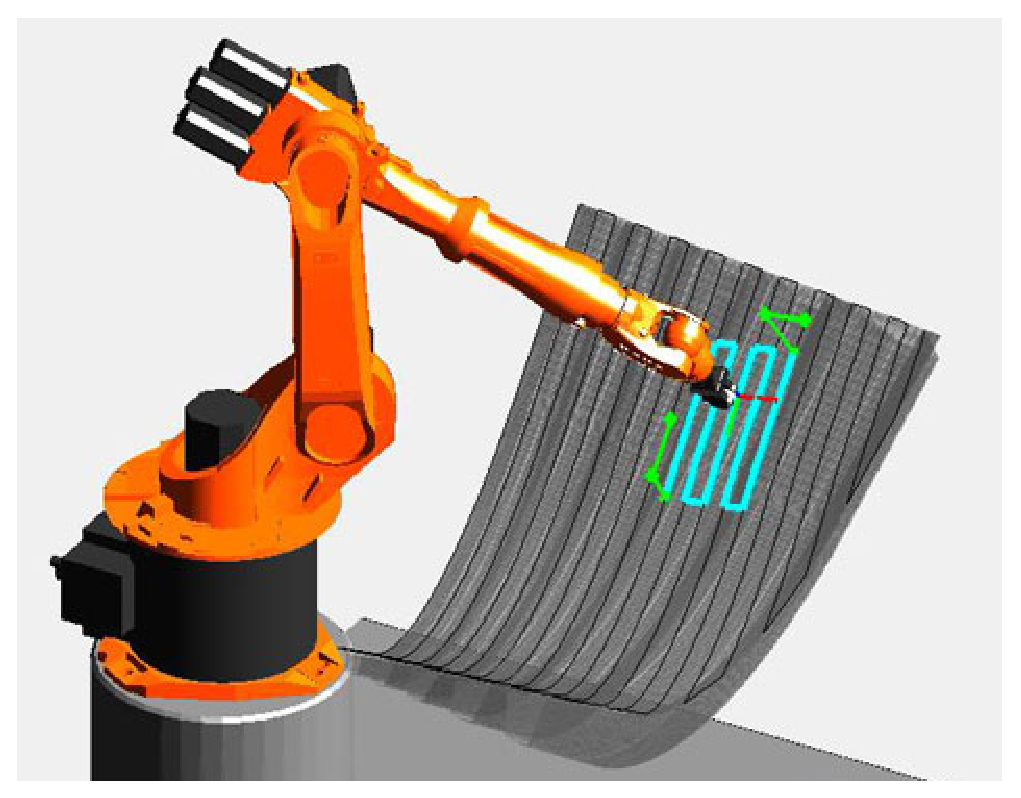
\includegraphics[scale=0.5]{img/chapter_1/example_coverage.eps}
	\vskip-15pt
	\caption*{\tiny twi-global.com}
	\caption{An example of an inspection coverage performed by a robotic arm.}
	\label{img:example_coverage}
\end{figure}

It is difficult to discuss good solutions to the coverage path planning problem because the notion of \emph{goodness} varies from one application to another. For example, a good coverage path for a painting robot would result in the most uniform paint layer on the surface. A good coverage path for a crop monitoring application would a yield high quality capture of the entire field. As such, works in literature that focus on one application offers solutions that are specialized to that application. On the other hand, numerous other works offer theoretical analysis and algorithmic approaches to the problem. These tend to propose solutions that theoretically achieve complete coverage; however, the solutions tend to posses undesirable properties such as excessive amount of turns that make their implementation in practice challenging.

In this work we aim to compute coverage paths with properties that make them desirable in practice by minimizing the amount of turns in the coverage path. Our key idea is to perform a line decomposition: an approximate decomposition of the workspace into regions that represent the area swept by the footprint traversing a straight line (Figure~\ref{fig:line_footprint}). The process starts with any convex decomposition. We propose a method of re-evaluating cuts in this convex decomposition with the objective of lowering the number of turns in the path. For each polygon in the final decomposition, a minimal line decomposition is performed. The complete coverage path is then generated by computing a tour of lines with minimal cost. Unlike existing approaches, the tour is not forced to complete local coverage of each polygon before proceeding to the next.

\begin{figure}
	\centering
	\subfile{img/chapter_1/line_footprint}
	\caption{Coverage footprint over a line.}
	\label{fig:line_footprint}
\end{figure}

Furthermore, this approach is used extensively in our extension to the multi-agent case. The key idea in the multi-agent case is to perform an assignment of regions to the team of $n$ robots with the goal of minimizing the maximum cost that includes the turning costs. The process starts with any $n$-cell decomposition. We propose a similar method of re-evaluating cuts in this decomposition with a new cost that includes turning costs. The result is a re-optimized $n$-cell decomposition where each cell represents assigned an area assigned to one of the $n$ robots. The coverage path for each robot is computed using the minimum turns decomposition approach.


\section{Thesis Contribution}
\label{section:thesis_contribution}

Our key contributions for the single-agent coverage are threefold. First, we provide a method for computing the minimum altitude of a non-convex polygon, which captures the number of parallel line segments, and thus turns, needed for coverage. Second, given an initial convex decomposition of a workspace, we propose a method to iteratively re-optimize and delete cuts of the decomposition in order to optimize the altitude of the polygon on each side of the cut. The proof of its correctness and computational complexity is provided. Third, we compute a coverage path of the workspace by placing parallel line segments in each region, and then computing a minimum-length tour of the corresponding approximate convex decomposition. The tour is computed by generating and solving a Generalized Traveling Salesman Problem (GTSP) instance using existing solvers.

The key contributions for the multi-agent coverage are twofold. First, we introduce a metric that assigns an approximation of the coverage cost that includes turning costs to a polygon. Second, given an initial $n$-cell decomposition of a workspace, we propose an iterative procedure for re-optimizing cuts of the $n$-cell decomposition in order to decrease the maximum coverage cost over all cells in the decomposition. The coverage path for each robot in the team is computed using the single-agent approach.

\section{Organization}
\label{section:organization}

The thesis is organized into six chapters. Chapter~\ref{chapter:literature_review} contains the literature review of single and multi-agent coverage works. Chapter~\ref{chapter:background} reviews some of the concepts used throughout this thesis. Chapter~\ref{chapter:single_agent_coverage} introduces our approach to the single agent coverage path planning problem. Chapter~\ref{chapter:multi_agent_coverage} introduces our approach to the multi-agent coverage path planning problem. Finally, Chapter~\ref{chapter:future_work} provides conclusion to this thesis and recommendations for avenues of future research.

\end{document}